\chapter{Application design and implementation}\label{sec:ApplicationDesingAndImplementation}
This chapter describes all important information about created application. First is hardware and software used for developing and testing of the application. Second is structure and description of core parts used in the application. 

\section{Hardware}\label{sec:Hardware}
There are three main Hardware components used and those are smartphone, smartwatch and BLE beacons. Both smart devices must support scanning of Bluetooth Low Energy beacons that can be done with Bluetooth 4.0 and higher. Secondary requirements are Wi-Fi, GSM and LTE modules to be able to scan more types of devices than just BLE beacons.  

% Maybe add beacons server information?

\subsection{Smartphone}\label{subsec:Smartphone}
Main part of the application will be developed and tested on Redmi Note 4 from Chinese company Xiaomi. It is running customized version of Android 6.0 called MIUI. Even thought system was customized in core it is still Android so there are no problems in that regard  \cite{XRN4LTE}. This phone has Bluetooth 4.1 with LE support so main requirement for the hardware is met. This device also met all the secondary requirements with Wi-Fi 802.11 a/b/g/n, GSM, and LTE support like most modern smartphones would \cite{XRN4FPS}.

\subsection{Smartwatch}\label{subsec:Smartwatch}
As already mentioned this thesis is using smartwatch with support of Android Wear 2.0 which makes it harder to select proper wear device since there not so many options at this time. There was around twenty of watches with 2.0 system and only five of them were selected to closer inspection based on few articles \cite{BAWW, BAWW18, BAWW17}.

\begin{table}[h]
	\scriptsize
	\begin{center}
		\begin{tabular}{| m{3cm} | c | c | l |}
			\hline
			Watch & BLE / Wi-fi & Czech Republic & Problems \\ \hline
			LG W280 Sport & Yes / Yes & No & \begin{tabular}[c]{@{}l@{}} Battery life is one day or less. \\ Too big in size. \end{tabular} \\ \hline
			LG W270 Titanium Style & Yes / Yes & Yes & Battery life is one day or less. \\ \hline
			Huawei Watch 2 & Yes / Yes & Yes & \begin{tabular}[c]{@{}l@{}} First update can take a long time. \\ Slight Bluetooth pairing issues. \end{tabular} \\ \hline
			Polar M600 & Yes / Yes & Yes & \begin{tabular}[c]{@{}l@{}} Polar support complains. \\ Phone synchronization issues. \\ GPS location malfunctions. \end{tabular} \\ \hline
			ASUS ZenWatch 3 & Yes / Yes & No &  \begin{tabular}[c]{@{}l@{}} Strap breaks fast. \\ AW 2.0 update can break the watch. \\ ASUS support complains. \end{tabular} \\ \hline
		\end{tabular}
		\caption{Smartwatch comparison (sources: \cite{LGWSP, LGWST, HW2, PM600, AZW3})}
		\label{tab2}
	\end{center}
\end{table}

There were funds only for one watch device out of five which is displayed in \tref{tab2} with selection parameters. First requirement for the wear device is support of BLE and Wi-Fi which all have. Second information considered was being able to buy it in Czech Republic (CR) since it is easier for prices, shipping and warranty. Only three of five devices were sold in CR at that time so others are out of the question. Final decision was made based on extensive research of customer reviews in shopping sites (Amazon, CZC, Heureka, Alza), wear official websites \cite{LGWSP, LGWST, HW2, PM600, AZW3} and other tech sites \cite{BAWW, BAWW18, BAWW17}. Finally, selected device is Huawei Watch 2 since there were not too many problems in reviews and other requirements were met. 

Initial setup of the wear device was composed of two main parts. First one was update wear system that took about one to two hours. Second task was copy Google account into the wear device where problem was discovered. Copying of accounts from Redmi Note 4 ti the watch hanged nd never completed. To fix this problem another smartphone was used to copy the account but as it was already mentioned only single device can be connected to smartwatch and connecting a new one requires factory reset that would remove all the data. So there was the need to pair wear with phone without factory reset which was handled via debugging following this \cite{HtPAWW} article.

\subsection{BLE beacons}\label{subsec:BLEBeacons}
Beacons are small devices that can be easily placed in almost any environment. The only thing they do is send their information packets using bluetooth and are used in museums, airports and as of late in indoor localization \cite{10TABB}. Beacons have their own battery that can last around a year without charging because of the new Bluetooth Low Energy (BLE) standard that consumes little to no energy \cite{IPSBOBLE}. 

There are multiple beacon manufacturers with their own quality, signal strength, battery life and other hardware differences. There are also multiple software (packet) specifications for beacons meaning that data they send have different format but they does not mean other systems cannot see them. Beacons are usually platform independent and work with multiple platforms \cite{IPSBOBLE, 10TABB}.

\begin{figure}[H]
	\begin{centering}
		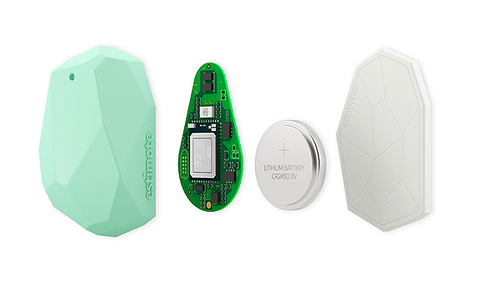
\includegraphics[width=0.6\textwidth]{img/estimote_beacon}
		\par\end{centering}
	\caption{Parts of Estimote beacon (source: \cite{RMPFEB})\label{fig:PartsOfEstimoteBeacon}}
	\label{fig10}
\end{figure}

Another important thing to note it that Beacons are not connected to the Internet and do not collect any data from devices around. Meaning all the data have to be processed in another device, most commonly a smartphone, and it also makes Beacon safe to use because there is no need to worry about sensitive data theft \cite{10TABB}.

\section{Software}\label{sec:Software}
Smart phone and wear use Android system which was already described in \hyperref[sec:Android]{Chapter 3}. This section will provide basic information about libraries, technologies and systems used in the application or supporting it.

\subsection{AltBeacon Library}\label{subsec:AltBeaconLibrary}
There are multiple solutions that can be used to scan for BLE beacons as for example Estimote SDK \cite{ESDKfA} which was already used in previous thesis \cite{PMRIL}. To change things up BLE beacons are found via AltBeacon Library \cite{ABL}.

Since there is no open and interoperable specification for proximity beacons, Radius Networks has authored the AltBeacon specification as a proposal for how to solve this problem. It is a open and free specification for Bluetooth Low Energy beacons with focus to create an open, competitive market for proximity beacon implementations \cite{AltB}.

This library enables Android devices to scan for iBeacons based on previously mentioned AltBreacon standard but it can be customized to support different kinds of beacons. It also supports Eddystone which is Google's open source beacon format and calculation of range between the devices which will help with localization \cite{ABL, EDDF}.

\subsection{Database}\label{subsec:Database}
Database is needed to keep all the Fingerprint data for calculations and there are two types of databases used for this application. First one is SQLite database that is used in Android application to save Fingerprints. This database is default and most used solution in Android applications and there is no need to use other ones. Another type of database used is Couchbase which is implemented on \verb|beacons.uhk.cz| server to keep all Fingerprint data on one place for multiple applications.

\subsubsection{Couchbase database}\label{subsec:CouchbaseDatabase}
Since SQL based databases can be complex to implement, scale and consuming more data storage space there was a drive to create so called NoSQL databases. Their most important feature is not having a scheme, that makes them easy to scale, and easy to replicate between multiple devices. There are around 225 NoSQL databases at this time and Couchbase is one of them \cite{NOSQLDB}.

Couchbase is distributed, document-based database with its own querying language called N1QL. It is a database focused on simple server configuration and easy use for clients and with built in caching layer and distribution system it does not require any changes in the application. There can be either one server instance of Couchbase or multiple of them can be connected and create a database cluster that holds all the data in multiple location (nodes) \cite{GSWCBS}.

Since SQL is used for decades and it became standard for working with data in databases this approach was extended for usage with JSON and called N1QL. It has all features of the SQL with only difference of being focused on JSON files that has no structure and it is used in Couchebase \cite{WINQL}.

There is a version of Couchbase for mobile called Lite that provides APIs to work with the documents and synchronize with the server instance. Problem of this solution is that Lite version does not implement N1QL and maps data as document views that have to instanced and usually use more data, at least on Android. 

\subsubsection{SQLite database}\label{subsec:SQLiteDatabase}
SQL (Structured Query Language) is a standard language for storing, manipulating and retrieving data in databases. It is a type of Relational Database that means all data is saved into tables with rows and columns \cite{ItSQL}. These tables usually have set amount of rows with specific names that protect from adding wrong data as en example you cannot add data \verb|Person(name, surname, eye color)| into table \verb|Person(name, surname)| because there is no column named \verb|eye color| in the table.

Advantages of these databases are structured data which makes calculation faster but uses more storage space. Data can be only saved once since they can be connected to each other. It supports complex queries for creating, reading, updating and removing data (CRUD) and better security with user and table management. Some disadvantages of this system can be with complexity and inflexibility of database scheme because it can be hard to setup and it does not allow other data then is defined in the tables \cite{ERDMS}.

Since SQL with all the features can consume a lot of hardware resources for a smartphone that is not as fast as a server Android decided to implement SQLite. SQLite has the following noticeable features: self-contained, serverless, zero-configuration, transactional \cite{WISQLITE}.

\begin{itemize}
	\item Serverless = does not need second process for the server.
	\item Self-Contained = requires minimal support from operating system.
	\item Zero-configuration = no need for installation or any configuration.
	\item Transactional = data are protected against failed changes (application crashes, power failure, ...).
\end{itemize}

\subsubsection{Comparison}\label{subsec:Comparison}
Both of these database solutions were tested on Android and SQL proved as a better solution. Not only it takes less storage space it is also able to load data faster. As \tref{tab3} shows SQL lite takes less data space and is almost three times faster in loading all the documents.

\begin{table}[h]
	\begin{center}
		\begin{tabular}{| l | c | c |}
			\hline
			Database type & Data size & Loading speed (315 documents) \\ \hline
			SQLite & 15MB & 23 second \\ \hline
			Couchbase without views & 31MB & 65 seconds \\ \hline
			Couchbase with views & 91MB & 65 seconds \\ \hline
		\end{tabular}
		\caption{Couchbase vs SQLite (sources: \cite{LGWSP, LGWST, HW2, PM600, AZW3})}
		\label{tab3}
	\end{center}
\end{table}

As shown SQL comes up better but it does not support any data synchronization so there must be custom solution created. If Couchbase Lite would have faster query time it would be preferable solution but it is not at this time.

\subsection{TileView}\label{subsec:TileView}
There are multiple ways to display map image in Android but the main ones have problems while displaying a big image because they will run out of memory. So it is usually better to try custom library or widget created specifically for displaying big image. There is multiple 2D and 3D libraries to display such an image but most of them display image as a whole meaning one big image file. 

There is another way introduced by Google Maps where map is displayed using small images so called \verb|tiles|. Image is cut into small pieces which is better for device memory management than one big image. Depending on how big the cuts are it can also display multiple zoom levels keeping the map quality high with high and low levels.

% Example of this and how to do it

\section{Application structure}\label{sec:ApplicationStructure}
This section describes structure of the applications and since there are two parts of this application (mobile and wear) both of them will be described.

\subsection{Mobile application}\label{subsec:MobileApplication}
Mobile application is the bigger and more complex part that handles scanning, map display and synchronization with the server.

\subsubsection{Activities}\label{subsec:Activities}
Activities are visible screens of the application. They serve as the entry point for a user's interaction with an application, and are also central to how a user navigates within an application (as with the Back button) or between apps (as with the Recents button) \cite{AD}.

Main activity for this application is called \verb|ScanActivity|. It displays map with proper building, floor and found Fingerprint in that specific location. It enables users to scan for new beacons and thus create new Fingerprints. Map and controls are implemented using TileView widget that was described in previous section. 

\subsubsection{Model}\label{subsec:Model}
Model package contains most important classes of the application and it's split into four parts called: adapters, configuration, database and tasks.

\paragraph{Adapters}\label{subsec:Adapters}\mbox{} \\
Adapters information. 

\paragraph{Configuration}\label{subsec:Configuration}\mbox{} \\
Configuration classes contain settings of the application. It uses Android's shared preferences that are key-value (xml) files to save small amount of application data. Each SharedPreferences file is managed by the framework and can be private or shared. One thing to note is that these files are not encrypted so it is not good to save user sensitive data in them.

\paragraph{Database}\label{subsec:Database}\mbox{} \\
Database package contains all classes needed for communication between application and SQL database. First part of this package are Fingerprints classes that correspond with tables and columns of the database. Second part are so called database helpers that handle communication between the application and SQLite database such as tables creation, selects, inserts, updates and deletions.

\paragraph{Tasks}\label{subsec:Tasks}\mbox{} \\
Tasks contain the most complex classes of this application and that is the Fingerprint scanner that has multiple sub-classes to parse all the necessary data from the scan. Tasks also contain connection with the server for data synchronization and Fingerprint transfers.

\subsubsection{Utilities}\label{subsec:Utilities}
Utilities contain classes not fit to any other category or classified as support ones which usually means classes for animations or warning messages but since this application communicates with the wear device this package also contains classes that handle such communication.

\subsection{Wear application}\label{subsec:WearApplication}
Wear application is simplified version of its smartphone counterpart. It handles only scanning, display of scanning progress and sending the data to the phone. 